\documentclass[tikz,border=5pt]{standalone}
\usepackage{luatexja}
\usepackage[hiragino-pron]{luatexja-preset}
\usepackage{amsmath,amssymb}
\usetikzlibrary{arrows.meta,patterns}

\begin{document}
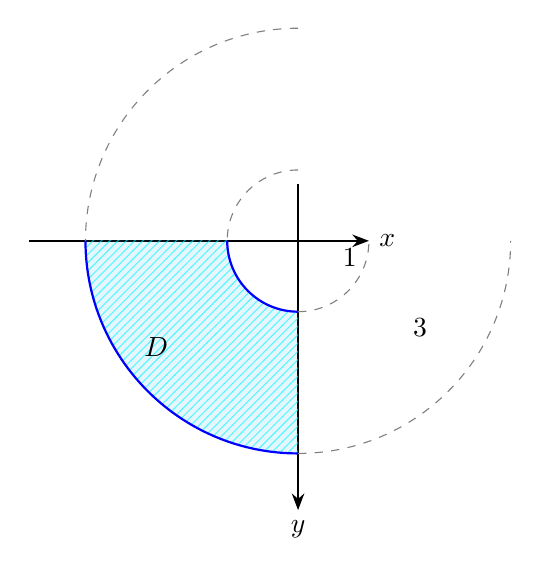
\begin{tikzpicture}[scale=0.9]

% Axes
\draw[-{Stealth[length=6pt]}, thick] (-3.8,0) -- (1,0) node[right] {$x$};
\draw[-{Stealth[length=6pt]}, thick] (0,0.8) -- (0,-3.8) node[below] {$y$};

% Fill annular region in third quadrant (r=1 to r=3)
\begin{scope}
  \clip (-3.5,-3.5) rectangle (0,0);
  \fill[pattern=north east lines, pattern color=cyan, opacity=0.6, even odd rule]
    (0,0) circle (3) (0,0) circle (1);
  \fill[cyan, opacity=0.1, even odd rule]
    (0,0) circle (3) (0,0) circle (1);
\end{scope}

% Circle boundaries (only third quadrant arcs)
\draw[thick, blue] ({1*cos(180)},{1*sin(180)}) arc (180:270:1);
\draw[thick, blue] ({3*cos(180)},{3*sin(180)}) arc (180:270:3);

% Dashed full circle hints
\draw[dashed, thin, gray] ({1*cos(270)},{1*sin(270)}) arc (270:360:1);
\draw[dashed, thin, gray] ({1*cos(90)},{1*sin(90)}) arc (90:180:1);
\draw[dashed, thin, gray] ({3*cos(270)},{3*sin(270)}) arc (270:360:3);
\draw[dashed, thin, gray] ({3*cos(90)},{3*sin(90)}) arc (90:180:3);

% Labels
\node[above right] at ({0.7*cos(315)},{0.7*sin(315)}) {$1$};
\node[above right] at ({2.1*cos(315)},{2.1*sin(315)}) {$3$};
\node at (-2,-1.5) {$D$};

\end{tikzpicture}
\end{document}
